    \subsection{Приложения теории гомологий}

    \begin{theorem}[Борсук]\label{BorsukTheorem}
        Не существует ретракции диска на граничную сферу.
    \end{theorem}
    \begin{proof}
        Предположим, что ретракция $f\colon D^n \to S^{n - 1}\colon f$~--- непрерывное и $f\vert_{S^{n - 1}} = \mathrm{id}$ существет.
        Рассмотрим отображение $i\colon S^{n - 1} \hookrightarrow D^n$, тогда в гомологиях у нас есть отображение
        \[ H_{n - 1}(S^{n - 1}) \xrightarrow{i_{*}} H_{n - 1}(D^n) \xrightarrow{f_{*}} H_{n - 1}(S^{n - 1}) \]
        или, подставляя известные нам результаты:
        \[ \Z \xrightarrow{i_*} 0 \xrightarrow{f_{*}} \Z. \]
        Так как $f \circ i = \mathrm{id}$, $f_* \circ i_* = \mathrm{id}_* = \mathrm{id}$ и мы приходим к противоречию.
    \end{proof}
    
    \begin{theorem}[Брауэр, о неподвижной точке]
        Пусть $f\colon D^n \to D^n$~--- непрерывное отображение. 
        Тогда у него существует неподвижная точка. 
    \end{theorem}
    \begin{proof}
        Предположим противное, пусть существует непрерывное $f\colon D^n \to D^n$, не имеющее неподвижных точек. Рассмотрим отображение $g$, которое переводит $x \in D^n$
        в точку пересечения $[f(x), x)$ и $\partial D^n$. То есть, $g\colon D^n \to \partial D^n$ и $g\vert_{\partial D^n} = \mathrm{id}$.
        Тогда $g$~--- ретракция $D^n$ на граничную сферу, а этого не бывает по теореме~\ref{BorsukTheorem}.
    \end{proof}
    
    \begin{theorem}[Брауэр, инвариантность размерности]
        Если непустые открытые $U \subset \R^m$, $V \subset \R^n$ открытые и они гомеоморфны, то $m = n$.
    \end{theorem}
    \begin{proof}
        Пусть $h$~--- гомеоморфизм $U \to V$, тогда
        \[ H_{k}(U, U - x) \cong H_{k}(V, V - h(x)). \]
        По теореме о вырезании~\ref{CuttingTheorem} для $(X, A) = (\R^m, \R^m - x)$ и $Z = \R^m - U$:
        \[ H_{k}(\R^m, \R^m - x) \cong H_{k}(U, U - x). \]
        Тогда мы имеем, что
        \[ H_{k}(\R^m, \R^m - x) \cong H_{k}(\R^n, \R^n - h(x)). \]
        Из точной последовательности пары для $(\R^m, \R^m - x)$ мы имеем:
        \[ \ldots \to H_{k}(\R^m) \to H^{k}(\R^m, \R^m - x) \to H_{k - 1}(\R^{m} - x) \to H_{k - 1}(\R^m) \to \ldots \]
        \[ \ldots 0 \to H^{k}(\R^m, \R^m - x) \to H_{k - 1}(\R^{m} - x) \to 0 \to \ldots, \]
        а значит, $H_{k}(\R^m, \R^m - x) \cong H_{k - 1}(\R^m - x) \cong H_{k - 1}(S^{m - 1})$, так как
        $\R^{m} - x$ деформационно ретрагируется на $S^{m - 1}$. Значит, мы получили
        \[ H_{k - 1}(S^{m - 1}) \cong H_{k - 1}(S^{n - 1}), \]
        откуда ясно, что $m = n$.
    \end{proof}

    \subsection{Симплициальные комплексы}

    \textcolor{ForestGreen}{Этот парагарф надо написать из Хатчера}.

    \subsection{Эквивалентность симплициальных и сингулярных гомологий}

    \noindent\bf{Образующая $H_{n}(S^n)$:}

    В этом параграфе будем обозначать $n$-мерный симплекс, как $\Delta^n$. Заметим, что так как $\Delta^n/\partial \Delta^n \cong S^n$, по теореме о факторизации~\ref{FactorizationTheorem}
    мы имеем изоморфизм
    \[ H_{n}\lr*{S^n}\cong H_n\lr*{\Delta^n, \partial \Delta^n}. \]

    Покажем, что образующая $H^{n}(S^n)$~--- это отображение $\Delta^n \xrightarrow{\mathrm{id}} \Delta^n$.
    Нетрудно заметить, что $\Im(\partial f) \subset \partial \Delta^n$, что дает нам, что $\mathrm{id}$ вообще
    представляет какой-то гомологический класс в $H_{n}\lr*{\Delta^n, \partial \Delta^n}$.

    Рассмотрим тройку $\lr*{\Delta^n, \partial \Delta^n, \Lambda}$, где $\Lambda$~--- это
    $\partial \Delta^n$ без одной из граней (например, запоолненный треугольник, граница треугольника и граница треугольника без стороны).
    Напишем точную последовательность тройки:
    \[ \ldots \to H_{n}\lr*{\partial \Delta^n, \Lambda} \to H_{n}\lr*{\Delta^n, \Lambda} \to H_{n}\lr*{\Delta^n, \partial \Delta^n} \to H_{n - 1}\lr*{\partial \Delta^n, \Lambda} \to H_{n - 1}\lr*{\Delta^n, \Lambda} \to \ldots  \]
    Заметим, что так как $\Delta^n$ деформационно ретрагируется на $\Lambda$, $H_{n}\lr*{\Delta^n, \Lambda} \cong H_{n}\lr*{\Lambda, \Lambda} = 0$ и то
    же самое справедливо для $(n - 1)$-х гомологий. То есть, наша последовательность на самом деле имеет вид
    \[ \ldots \to  0 \to H_{n}\lr*{\Delta^n, \partial \Delta^n} \to H_{n - 1}\lr*{\partial \Delta^n, \Lambda} \to 0 \to \ldots  \]
    Теперь заметим, что если грань, которую мы выкинули, мы обозначим за $\Delta'$, то $H_{n - 1}\lr*{\partial \Delta^n, \Lambda} \cong H_{n - 1}\lr*{\Delta', \partial \Delta'}$.

    Это ценно, так как далее мы можем рассуждать по индукции, ведь если образующая $H_{n - 1}\lr*{\Delta', \partial \Delta'}$~--- вложение выкинутой нижней грани $\Delta'$, то
    её прообраз в $H_{n}\lr*{\Delta^n, \partial \Delta^n}$~---- нужное нам тождественное отображение (мы тут пользуемся тем, что
    мы знаем, что связывающий гомоморфизм в длинной точной последовательности пары/тройки~-- это просто взятие границы). А для $S^0$ это утверждение очевидно.

    Обозначим симплиаицльные гомологии пространства $X$ за $H_{k}^{\Delta}(X)$.
    \begin{theorem}
        Пусть $X$~--- конечный симплициальный комплекс. Тогда
        \[ H_{k}^{\mathrm{sing}}(X) \cong H_{k}^{\Delta}(X). \]
    \end{theorem}
    \begin{proof}
        Пусть $X^k$~--- объединение всех симплексов в симплициальном комплексе до размерности $k$ (обозначение аналогично обозначению для $\mathrm{CW}$-комплексов).
        Напишем точную последовательность пары:
        \[ \ldots \to H_{n + 1}^{\Delta}\lr*{X^k, X^{k - 1}} \to H_{n}^{\Delta}\lr*{X^k} \to H_{n}^{\Delta}\lr*{X^k} \to H_{n}^{\Delta}\lr*{X^k, X^{k - 1}} \to \ldots \]
        и заметим, что $H_{n + 1}^{\Delta}\lr*{X^k, X^{k - 1}} \cong H_{n + 1}\lr*{X^k, X^{k - 1}} \cong H_{n + 1}\lr*{\bigvee S^k}$. Действительно, ясно, что
        \[ H_{n + 1}\lr*{X^k, X^{k - 1}} \cong H_{n + 1}\lr*{\bigvee_{\alpha}S^k}, \]
        где $\alpha$ пробегает $k$-мерные симплексы в $X$. Далее,
        \[ H_{n + 1}\lr*{\bigvee_{\alpha}S^k} \cong \begin{cases} 0, \quad \text{ если } n + 1 \neq k \\ \bigoplus_{\alpha} \Z, \quad n + 1 = k \end{cases}\]

        С другой стороны, из определения симплициальных гомологий ясно, что при $n + 1 \neq k$ мы имеем
        $H_{n + 1}^{\Delta}\lr*{X^k, X^{k - 1}} \cong 0$, а при $n + 1 = k$ эта группа~--- свободная абелева группа, порожденная
        всеми $k$-мерными симплексами в $X$, то есть, как и в предыдущем случае
        \[ H_{k}^{\Delta}\lr*{X^k, X^{k - 1}} \cong \bigoplus_{\alpha} \Z. \]
        Остается заметить, что по доказанному в начале параграфа, мы знаем, что у $H_{k}\lr*{\bigvee_{\alpha} S^k}$ такой же набор порождающих.

        Теперь будем вести индукцию по размерности симплициального комплекса. По индукционному предположению мы имеем
        $H_{n}^{\Delta}(X^{k - 1}) \cong H_{n}(X^{k - 1})$ и тогда мы получаем диаграмму из 5-леммы:

        \begin{center}
            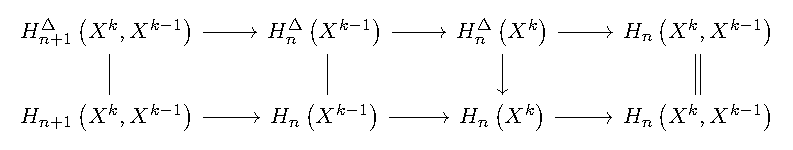
\includegraphics{lectures/0/pictures/cd_9}
        \end{center}
    \end{proof}

    \subsection{Степень отображения}

    \begin{definition}
        Пусть $f\colon S^n \to S^n$~--- непрерывное отображение. Тогда оно индуцирует морфизм в гомологиях:
        \[ f_{*}\colon H_{n}\lr*{S^n} \to H_{n}\lr*{S^n}. \]
        Так как $f_{*}$~--- гомоморфизм бесконечной циклической группы в себя, он должен иметь вид
        \[ f_{*}(\alpha) = d \cdot \alpha \]
        для некоторого фиксированного $d \in \Z$, зависящего только от $f$. Это число называют \emph{степенью отображения $f$}
        и обозначают $\deg{f}$.
    \end{definition}

    \noindent\bf{Базовые свойства степени.}

    \begin{enumerate}
        \item $\deg{\mathrm{id}_{S^n}} = 1$.
        \item Если $f$~--- не сюръекция, то $\deg{f} = 0$, так как мы можем выбрать $x \in S^n\setminus f\lr*{S^n}$  и
        представить $f$ в виде композиции
        \[ S^n \to S^n \setminus \{ x \} \hookrightarrow S^n, \]
        а пространство $S^n \setminus \{ x \}$~--- стягиваемо, значит $H_{n}\lr*{S^n \setminus \{ x \}} = 0$, а значит и $f_{*} = 0$.
        \item Если $f \sim g$, то $\deg{f} = \deg{g}$.
        \item $\deg{f \circ g} = \deg{f} \cdot \deg{g}$.
        \item Если $f$~--- гомотопическая эквивалентность,  то существует $g$ такое, что $f \circ g \sim \mathrm{id} \Rightarrow \deg{f} \deg{g} = 1 \Rightarrow \deg{f} = \pm 1$.
        \item Рассмотрим $f$, которое тождественно действует на первых $n$ координатах и отправляет $x_{n + 1}$ в $-x_{n + 1}$.
        Тогда $\deg{f} = -1$.  Действительно, мы модем реализовать сферу, как склейку двух симплексов $\Delta_{1}^n$ и $\Delta_{2}^n$ по границе.
        Тогда $n$-мерная цепь $\Delta_1^n - \Delta_2^n$ являются образующей $n$-мерных гомологий, а отображение $f$ переставляет местами
        $\Delta_1^n$ и $\Delta_2^n$, то есть действует на образующую умножением на $-1$.
        \item Степень антиподального отображения: $\deg\lr*{x \mapsto -x} = (-1)^{n + 1}$
        \item Если $f \colon S^n \to S^n$ не имеет неподвижных точек, то $f \sim \lr*{x \mapsto -x}$ и соответственно $\deg{f} = (-1)^{n + 1}$.  Действительно, если $f(x) \neq x$, то
        отрезок с концами $f(x)$ и $-x$, который задаётся, как
        \[ t \mapsto (1 - t)f(x) - tx, \ 0 \le t \le 1, \]
        не проходит через начало координат и формула
        \[ H(t, x) = \frac{(1 - t)f(x) - tx}{\| (1 - t)f(x) - tx \|} \]
        определяет гомотопию $f(x)$ в постоянное отображение.
    \end{enumerate}

    \begin{theorem}[О причёсывании ежа]
        $S^n$ допускает непрерывное ненулевое (касательное) векторное поле тогда и только тогда, когда $n$~--- нечетно.
    \end{theorem}
    
    \begin{proof}
        Предположим, что $x \mapsto V(x)$~--- непрерывное поле касательных векторов к сфере. Тогда,
        если рассматривать вектор $V(x)$, как вектор в начале координат, а не в точке касания, то условие касания означает просто, что
        $x \perp V(x)$. Если $V(x) \neq 0$, то мы можем нормализовать веторное поле так, что $\| V(X) \| = 1 \ \forall x$, тогда векторы
        \[ (\cos{t})x  + (\sin{t})V(x) \]
        лежат на единичной окружности в $\Span\lr*{x, V(x)}$.
        Соотвественно, при $t \in [0, \pi]$  мы получаем гомотопию тождественного отображения $\mathrm{id}_{S^n}$ в антиподальное отображение:
        \[ H(t, x) = (\cos{t})x  + (\sin{t})V(x). \]
        Отсюда следует, что $(-1)^{n + 1} = 1$, а значит, $n$ должно быть нечетно. С другой стороны, когда $n = 2k - 1$, мы можем положить
        \[ V(x_1, x_2, \ldots, x_{2k - 1}, 2k) = (-x_2, x_1, \ldots, - x_{2k}, x_{2 k + 1}) \]
        и это даст нам искомое векторное поле.
    \end{proof}

    Опишем теперь метод вычисления, который чаще всего применим на практике.
    Пусть $f\colon S^n \to S^n$ и существует $y \in S^n$ такое, что $f^{-1}(y) = \{ x_1, \ldots, x_k \}$,
    $U_1, \ldots, U_k$~---  непересекающиеся окрестности этих точек, которые $f$ переводит в  окрестность $V$ точки $y$.
    Тогда $f\lr*{U_i \setminus x_i} \subset V \setminus y$ и мы имеем коммутативную диаграмму:
    \begin{center}
        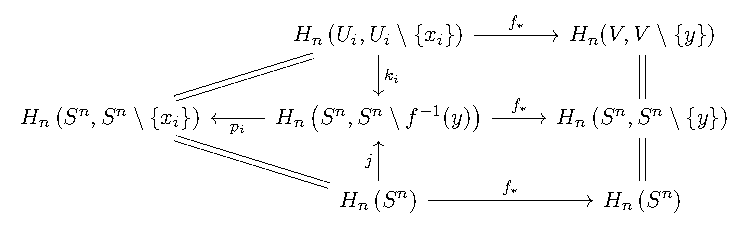
\includegraphics{lectures/0/pictures/cd_10}
    \end{center}

    Все отображения на ней индуцируются включениями. Два ихоморфизма в верхней части диаграммы получаются из теоремы о вырезании~\ref{CuttingTheorem},
    а два в нижней~--- из точной последовательности пары~\ref{LongExactSequenceOfPair}.

    Посредством этих четырех гомоморфизмов две верхние группы можно отождествить с $\Z$, тогда верхний
    гомоморфизм $f_{*}$ становится умножением на число и это число мы будем называть \emph{локальной степенью} отображения $f$
    и обозначать $\deg{f\vert_{x_i}}$.


    \begin{theorem}[Локальность степени]
        Пусть $f\colon S^n \to S^n$ и $y \in S^n$ таково, что $f^{-1}(y) = \{ x_1, \ldots, x_k \}$. Тогда
        \[ \deg{f} = \sum_{i} \deg{f}\vert_{x_i}.\]
    \end{theorem}
    \begin{proof}
        По теореме о выразении~\ref{CuttingTheorem}, группа $H_{n}\lr*{S^n, S^n \setminus f^{-1}(y)}$~--- прямая сумма групп
        $H_{n}\lr*{U_i, U_i \setminus \{ x_i \}}$,  причем $k_i$~--- отображение включения $i$-го слагаемого, а $p_i$~--- проекция на $i$-е слагаемое.
        Из коммутативности нижнего треугольника мы получаем, что
        \[ p_i \circ j (1) = 1, \]
        а значит, $j(1) = (1, \ldots, 1) = \sum_{i} k_i(1)$. Коммутативность верхнего квадрата говорит, что $f_*$ отображает $k_i(1)$ в $\deg{f\vert_{x_i}}$,
        а коммутативность нижнего квадрата уже дает нам формулу
        \[ \deg{f} = \sum_{i} \deg{f\vert_{x_i}}. \]
    \end{proof}